\chapter{Simulation results in 2D space}
Simulation of system $\dot{x}=f(x,u)$ defined by (\ref{eq:uni1}, \ref{eq:uni2}, \ref{eq:uni3}), with initial conditions $x(t_0)=[x_v, y_v, \theta_v]$ and initial input $u(t_0)=[u_s,u_{\omega}]$ has been implemented in Matlab  and Simulink. This chapter discuss various situations and two avoidance approaches. Control strategy $\Omega$ with voting algorithm $\gamma$ has been proposed in (\ref{eq:avoidanceStrategy})

\section{Simulation setup}
Simulation can be parametrized, simulation parameters are given in table \ref{tab:simulationparameterss}. During various simulation runs some parameters may be overridden if that happens then it will be denoted in simulation chapter as change of initial parameters. 
\begin{table}[H]
    \centering
    \begin{tabular}{|r|c|c|l|}
        \hline
        Parameter & Variable & Value & Units \\
        \hline
        \hline
        Input speed & $u_s$ & 1 & $[ms^{-1}]$ \\
        \hline
        Input turn & $u_{\omega}$ & 0 & $ [rad.s^{-1}] $ \\
        \hline
        Initial $x$ position & $x_v$& 0& $[m]$ \\
        \hline
        Initial $y$ position & $y_v$& 0& $[m]$ \\
        \hline
        Initial vehicle heading & $\theta_v$& $\pi/2$ & $[rad]$ \\
        \hline
        Maximal vehicle speed & $v_{max}$ & 1 & $[ms^{-1}]$ \\ 
        \hline
        Maximal vehicle turn & $u_{\omega max}$ & $\pi/12$ & $ [rad.s^{-1}] $ \\
        \hline
        Decision time & $t_{step}$ & 1 & $[s]$\\
        \hline
        Decision distance & $d_{step}$ & $v_{max}.t_{step}$ & $[m]$\\
        \hline
    \end{tabular}
    \caption{Initial simulation parameters}
    \label{tab:simulationparameterss}  
\end{table}


\subsection{Conservative approach}\label{s:conservativeapproach}
Conservative approach is based on following idea: "Vehicle always needs to have space to turn". Therefore control strategy $\Omega$ is reduced to set containing only maximum turn movements and voting algorithm $\gamma$ is formulated as follow:

\begin{algorithm}[H]
Define $\mathscr{D}$ as threat set from definition \ref{def:threatset} \;
Define $s_{turn} \in \{\textnormal{left},\textnormal{right}\}$ as turning side, $\gamma$=rand(\{left, right\})\;
\While{$\mathscr{D}!=\emptyset,\exists o_i \in\mathscr{D}:\delta_o==1$}{
    $u(t)=
    \begin{bmatrix}
        u_s\\
        s_{turn}.u_{\omega max}
    \end{bmatrix}
    $\;
}
\end{algorithm}
Defined control is saying, if there is threat which is in front of vehicle, keep turning, until vehicle are facing away from all threats. Only one things remains and it is definition of crash distance function from definition \ref{def:crashdistance}. Goal is to simulate turns of vehicle under starting heading $\theta_0\in(-\pi,\pi]$ (fig. \ref{fig:SimulatedTrajectioriesForDifferentTheta}), then approximate given set bondary by ellipse function (fig \ref{fig:15_ReachSetBoundary}).


\begin{figure}[H]
    \begin{subfigure}{0.5\textwidth}
    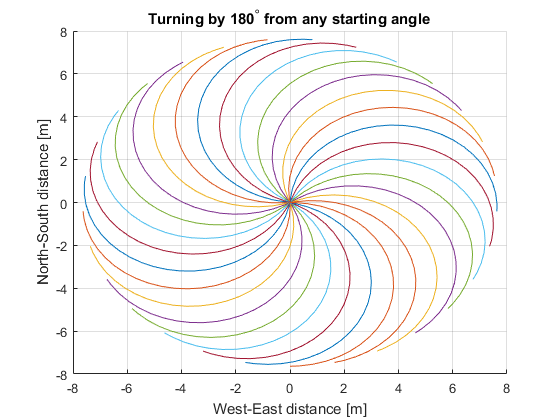
\includegraphics[width=0.9\linewidth]{\FIGDIR/14_Simulated_trajectiories_for_different_theta.png} 
    \caption{Simulated trajectiories for different $\theta$}
    \label{fig:SimulatedTrajectioriesForDifferentTheta}
    \end{subfigure}
    \begin{subfigure}{0.5\textwidth}
    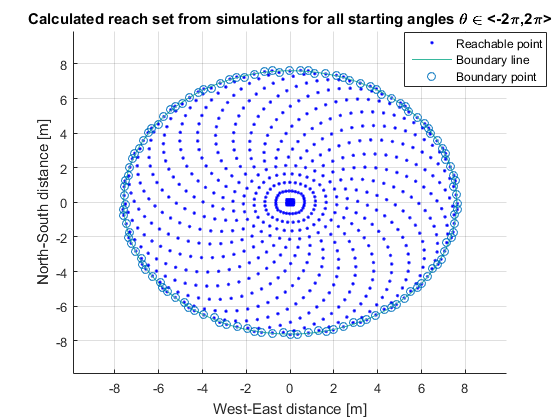
\includegraphics[width=0.9\linewidth]{\FIGDIR/15_Reach_set_boundary.png}
    \caption{Reach set boundary approximation}
    \label{fig:15_ReachSetBoundary}
    \end{subfigure}
\caption{Definition of maximal reach set at its boundary $\theta \in (-\pi,\pi>$}.
\label{fig:MaximalReachSet}
\end{figure}

Ellipse curve is defined by following equation:
\begin{equation}\label{eq:eclipseCurve}
    ax^2 + bxy + cy^2 + dx+ ey + f = 0\\
\end{equation}
Parameters for ellipse are given by ellipse direct fit algorithm \cite{fitzgibbon1999direct} and for given reach set they have following parameters: $a=017$, $b\approx0$, $c=0.0173$, $d\approx0$, $e\approx0$, $f=-1$. Because parameters $b, d, e$ are close to 0, it means that (\ref{eq:eclipseCurve}) can be replaced with circle equation in common (\ref{eq:circlecommon}) and parametrized (\ref{eq:circleparam}) form.

\begin{equation}\label{eq:circlecommon}
    (x - x_{off})^2 + (y-y_{off})^2 = r^2
\end{equation}
\begin{equation}\label{eq:circleparam}
    x^2 + y^2 = r^2; r=7.9
\end{equation}
What is remaining is definition of crash distance function $f(o,\vec{x}(t),\mathscr{O})$, safety margin $s_m$ must be taken into account (\ref{eq:safetymargin}), therefore function is given by:
\begin{equation}\label{eq:conservativecrashfunction}
    d_c = f(o,\vec{x}(t),\mathscr{O}) = 7.9 + s_m;
\end{equation}
Given crash distance function (\ref{eq:conservativecrashfunction}) is not very satisfactory, because it is very conservative. It is possible to make vehicle move closer to obstacles, but it requires more complicated voting algorithm $\gamma$ and more flexible crash distance function. Example of such approach is given in  section \ref{sec:smartinvariance}.

\subsection{Smart avoidance approach}\label{sec:smartinvariance}
Smart avoidance approach is based on following idea: "When vehicle approaches obstacle in front of it it must be avoided in distance appropriate to obstacle heading angle $\theta_b$". This idea seems strong in a first place, but practical testing shown, that, there is also other principle: "If there exist obstacle which is in vehicle close proximity away from heading angle $\theta$, i need to keep distance for possible turn". Obstacle heading/bearing angle $\theta_b$ is defined in (\ref{eq:obstacleHeadingAngle}) and belongs to range $(-\pi,\pi]$, obstacles in front of vehicle are those,where $\theta_b\in[-\frac{\pi}{2},\frac{pi}{2}]$, obstacles at back of vehicle are those, where $\theta_b \in \left\{(-\pi,-\frac{pi}{2})\cup(\frac{pi}{2},\pi]\right\}$.

\begin{figure}[H]
    \begin{subfigure}{0.5\textwidth}
    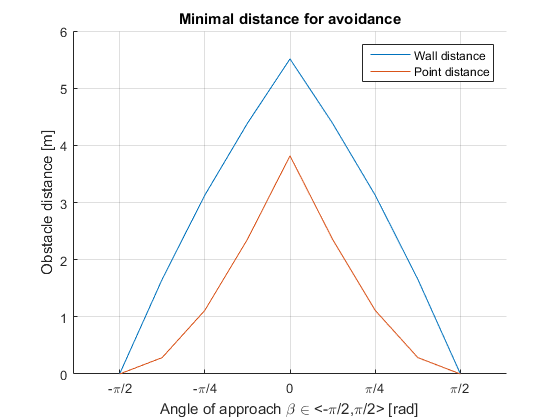
\includegraphics[width=0.9\linewidth]{\FIGDIR/12_Minimal_avoidance_distance.png} 
    \caption{Minimal avoidance distance for $\beta$}
    \label{fig:MinimalAvoidanceDistance}
    \end{subfigure}
    \begin{subfigure}{0.5\textwidth}
    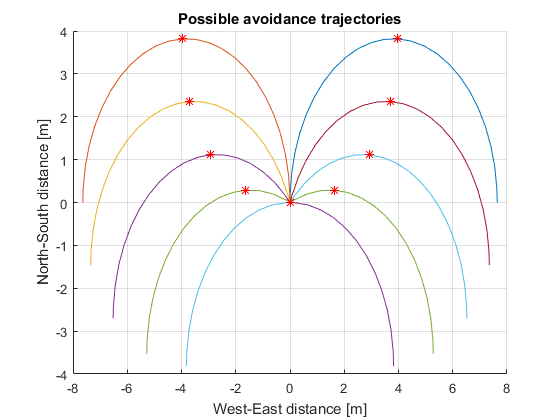
\includegraphics[width=0.9\linewidth]{\FIGDIR/13_Possible_avoidance_trajectories.png}
    \caption{Possible avoidance trajectories}
    \label{fig:PossibleAvoidanceTrajectories}
    \end{subfigure}
\caption{Definition of minimal avoidance distances $\beta$, based on obstacle type and obstacle heading angle $\theta_b \in [-\pi/2,\pi/2]$}
\label{fig:MinimalAvoidanceDistancesSmart}
\end{figure}


\begin{table}[H]
    \centering
    \begin{tabular}{|r||c|c|c|c|c|c|c|c|c|}
        \hline
        \twolinecellr{Obstacle heading\\ angle [rad]} & $-\frac{\pi}{2}$ & $-\frac{3\pi}{8}$ & $-\frac{\pi}{4}$ & $-\frac{\pi}{8} $ & $0$    & $\frac{\pi}{8}$ & $\frac{\pi}{4}$ & $\frac{3\pi}{8}$ & $\frac{\pi}{2}$ \\
        \hline
        Wall distance [m]       &     0	&  1.66 &  3.13	&  4.38 & 5.51 & 4.38 & 3.13 & 1.66	& 0 \\
        \hline
        Point distance [m]      &     0	&  0.29	&  1.11 &  2.35 & 3.82 & 2.35 &	1.11 & 0.29	& 0\\
        \hline
    \end{tabular}
    \caption{Avoidance distances for selected obstacle heading angle $\theta_b$}
    \label{tab:avoidanceDistances}
\end{table}

Crash distance $d_c$ for obstacle heading angle $\theta_b \in [-\frac{\pi}{2},\frac{\pi}{2}]$ is given by minimal avoidance distance function $/beta$ on figure \ref{fig:MinimalAvoidanceDistance}. Minimal avoidance distance function $\beta$ is heuristical function, which is looking a look-up table to find aproperiate distance for angle $\theta_b$. Interval of $\theta_b$ has been divided into 120 exact steps, for each step wall distance and point distance has been calculated. Let $\vec{x}_c = [x_c,y_c]$ be a northernmost point of trajectory for selected $\theta_b$ and $\vec{x}_p=[0,0]$ starting position of avoidance maneuver. Formula for point distance $d_{point}$ is given by (\ref{eq:pointdistance})and formula for wall distance $d_{point}$ is given by (\ref{eq:walldisance}).
. After all measurements, heuristic look-up function can be constructed as maximum median look-up on table \ref{tab:avoidanceDistances} given by equation (\ref{eq:betalookup}). Back of the vehicle is covered by previously defined maximal avoidance function from conservative approach (\ref{eq:conservativecrashfunction}), because in terms of avoidance vehicle needs to have place for full turn to avoid obstacles behind its back. Final crash distance function is given by (\ref{eq:smartdistancefunction}).

\begin{equation}\label{eq:pointdistance}
    d_{point} = x_c
\end{equation}
\begin{equation}\label{eq:walldisance}
    d_{wall} = \|\vec{x}_c\|
\end{equation}
\begin{equation}\label{eq:betalookup}
    \beta(\theta_b,\textnormal{type})=\textnormal{lookup}(\theta_b,\textnormal{type})
\end{equation}
\begin{equation}\label{eq:smartdistancefunction}
d_c = f(o,\vec{x}(t),\mathscr{O}) =
    \begin{cases}  
      \beta(\theta_b,\textnormal{type}) +s_m & \theta_b\in[-\frac{\pi}{2},\frac{\pi}{2}]\\
      7.9 + s_m  & \theta_b \in \left\{(-\pi,-\frac{pi}{2})\cup(\frac{pi}{2},\pi]\right\}
   \end{cases}
\end{equation}
What remains to define is voting algorithm $\gamma$, which will determine avoidance direction. Notable threats are incorporated in threat set $\mathscr{D}$ have local coordinates $[x_{o,i},y_{o,i}]$ in known world $\mathscr{F}$. The idea behind voting algorithm $\gamma$ is simple: "Go to the direction where is lesser threat for collision". To achieve this, it is required to divide dangers into two groups, dangers on the left plane and the dangers on the right plane. First step is to rotate dangers into alignment with plane heading $\theta_v$. Using standard rotation matrix on threat set $\mathscr{D}$ by equation (\ref{eq:rotationThreatSet}), one can get $\bar{\mathscr{D}}$. For each augmented threat $\bar{d}_i$ it is possible to calculate relative angle $\bar{\theta}_{b,i}\in(-\pi,\pi]$, which is given by (\ref{eq:relativeangletheta}).
\begin{equation}\label{eq:rotationThreatSet}
    \bar{\mathscr{D}}=
    \begin{bmatrix}
    \cos\theta_v&-\sin\theta_v\\
    \sin\theta_v&\cos\theta_v
    \end{bmatrix}
    \begin{bmatrix}
    x_{o,1}&\dots&x_{o,n}\\
    y_{o,1}&\dots&y_{o,n}
    \end{bmatrix}:
    \bar{d_i}\in\bar{\mathscr{D}},
    \begin{bmatrix}
    \bar{x}_{o,i}\\
    \bar{y}_{o,i}
    \end{bmatrix}
    \in \bar{d}_i 
\end{equation}
\begin{equation}\label{eq:relativeangletheta}
    \bar{\theta}_{b,i} = \arctan\left (\frac{\delta y_i}{\delta x_i}\right):\delta y_i = \bar{y}_{o,i} - y_v, \delta x_i = \bar{x}_{o,i} - x_v
\end{equation}
Voting algorithm $\gamma$ applied on control strategy $\Omega$ goes like follow: If threat set $\mathscr{D}$ is empty then fly straight otherwise fly to direction where are more votes. Algorithm can be summarized as follow: 

\begin{algorithm}[H]
\eIf{$\mathscr{D}!=\emptyset$}{
    left = count($\bar{d}_i\in\bar{\bar{\mathscr{D}}}$,$\bar{\theta}_{b_i}\le 0$)\;
    right = count($\bar{d}_i\in\bar{\bar{\mathscr{D}}}$,$\bar{\theta}_{b_i}> 0$)\;
    \eIf{left $\ge$ right}{
        $\omega(t)=\frac{\pi}{12}$\;}{
        $\omega(t)=-\frac{\pi}{12}$\;
        }
    }{
        $\omega(t)=0$\;
    }
\end{algorithm}


\section{Test plan}\label{s:testplan}
Purpose of testing is to prove capabilities of avoidance system, therefore test cases must cover critical situations,like crashes, corner avoidance, decisive situations, like testing of voting algorithm $\gamma$ to turn left or right, and long term simulations to test multiple obstacle avoidance scenarios.

Testing playground is metaphor to "fly in plastic box". Example of testing playground can is seen on figure \ref{fig:Playground}, where green stars represents \textit{obstacles}, red stars represent \textit{possible collisions}, yellow stars represents \textit{possible blockers} in case of turning, \textit{trajectory} is represented as blue line, red dots on trajectory represents \textit{runs of avoidance} during flight and pink squares on trajectory represents \textit{decision points}(avoidance start, avoidance end). 

\begin{figure}[H]
    \centering
    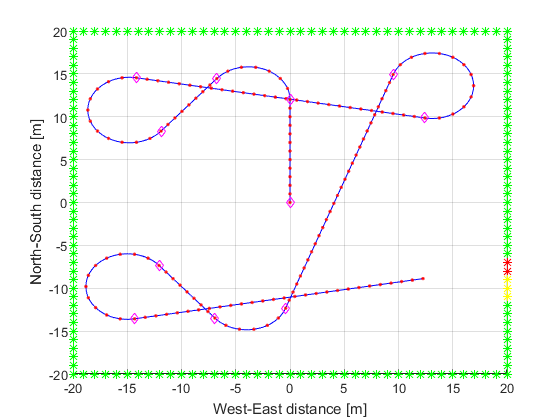
\includegraphics[width=0.9\linewidth]{\FIGDIR/16_Playground.png} 
    \caption{Testing playground}
    \label{fig:Playground}
\end{figure}

Testing cases can be defined as follow:
\begin{enumerate}
    \item \textit{Narrow wall avoidance} - vehicle is approaching wall straightforward, purpose of this test is to test basic avoidance, positive case is when vehicle avoids wall and heads back to box.
    \item \textit{Left slide avoidance} - vehicle is approaching wall from left, purpose of this test is to test voting algorithm if it chooses correct turn direction, positive case is when vehicle starts turning to approach direction.
    \item \textit{Right slide avoidance} - vehicle is approaching wall from right, purpose of this test is to test voting algorithm if it chooses correct turn direction, positive case is when vehicle starts turning to approach direction.
    \item \textit{Corner avoidance} - vehicle is approaching corner formation of playground, purpose of this test is to test corner avoidance, positive case is when vehicle avoids corner and heading inside of playground.
    \item \textit{Long term avoidance} - vehicle moves for longer period of time, this case generates long movement path, purpose of this test is to test combinations of previous cases and algorithm stability, positive case is when vehicle stays in box (forever).
\end{enumerate}

\newpage
\section{Simulation runs}\label{s:simulationruns}
Simulation runs have been executed according to test plan from section \ref{s:testplan}, control strategy $\Omega$ and voting algorithm $\gamma$ for experiment is defined by equation (\ref{eq:avoidanceStrategy}) and in chapter \ref{sec:smartinvariance}. During experiments following parameters were observed:
\begin{enumerate}
    \item \textit{State evolution} - evolution of vehicle trajectory among x and y axes represented by signals $x(t)$ and $y(t)$ and evolution of vehicle heading, represented by signal $\theta (t)$.
    \item \textit{Decision moments} - \textit{obstacle detection}, first obstacle detection in known space $\mathscr{F}$, this results into limitation of control strategy $\Omega$ to execute left or right turns, \textit{avoidance execution} or simple avoidance is stage in middle of execution snapshot vehicles situation during turning, control strategy $\Omega$ is still limited to left or right turns, \textit{end of avoidance} is phase when all dangerous obstacles are behind vehicle and control strategy $\Omega$ is returned to full set (vehicle continues to fly straight in given heading $\theta$).
    \item \textit{Voting algorithm results} - decision during obstacle avoidance is made based on voting algorithm $\gamma$, decision is made every algorithm run defined by $t_{step}$. Results are summarized in \textit{decision tables} for simple avoidance maneuvers.
\end{enumerate}

\subsection{Narrow wall avoidance}

\begin{figure}[H]
    \begin{subfigure}{0.5\textwidth}
    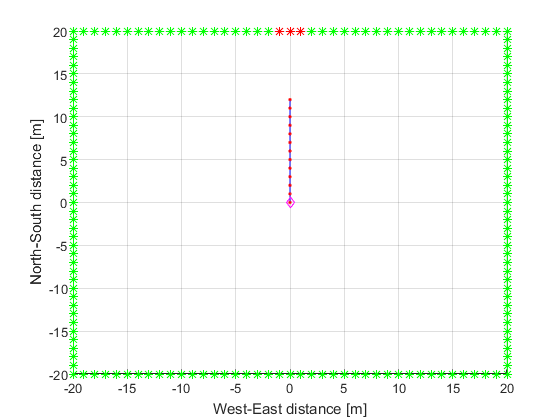
\includegraphics[width=0.9\linewidth]{\FIGDIR/17_Obstacle_detection.png} 
    \caption{Obstacle detection}
    \label{fig:17Obstacledetection}
    \end{subfigure}
    \begin{subfigure}{0.5\textwidth}
    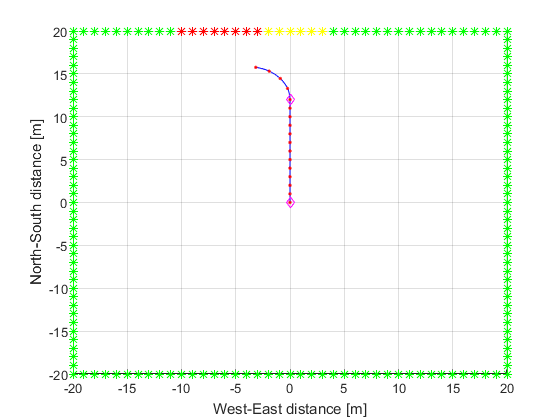
\includegraphics[width=0.9\linewidth]{\FIGDIR/18_Avoidance.png}
    \caption{Avoidance}
    \label{fig:18Avoidance}
    \end{subfigure}
    \\
    \begin{subfigure}{0.5\textwidth}
    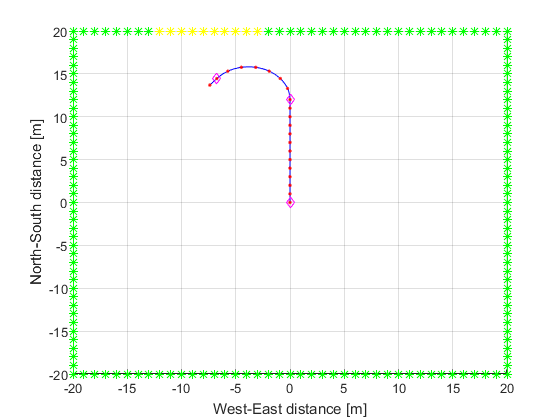
\includegraphics[width=0.9\linewidth]{\FIGDIR/19_End_of_avoidance.png} 
    \caption{End of avoidance}
    \label{fig:19Endofavoidance}
    \end{subfigure}
    \begin{subfigure}{0.5\textwidth}
    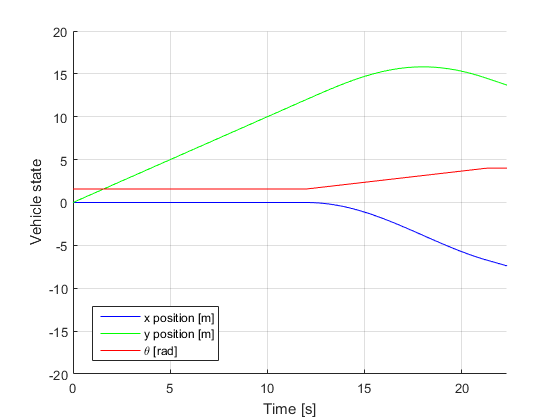
\includegraphics[width=0.9\linewidth]{\FIGDIR/20_Flight_parameters.png}
    \caption{Flight parameters}
    \label{fig:20Flightparameters}
    \end{subfigure}
\caption{Simulation result for narrow wall avoidance}
\label{fig:SimulationNarrowWall}
\end{figure}
Starting parameters $x_v = 0$, $y_v = 0$, $\theta_v = \pi/2$ have been used in addition to given initial conditions of simulation. Vehicle detects three possible obstacles (\ref{fig:17Obstacledetection}), because there exist threat of first type, control strategy $\Omega$ is limited to turn left or right. Voting algorithm $\gamma$ is taken into consideration and first decision is to turn left, because left side is favoured in terms of $\bar{\theta}_b=0$. Avoidance maneuver (\ref{fig:18Avoidance}) is executed until threat set $\mathscr{D}$ is not empty or exist threat $o_i$ in front of vehicle $\delta_o=1$. Avoidance ends when all threats $o_i\in\mathscr{D}$ are behind vehicle heading $\theta(t)$ (\ref{fig:20Flightparameters}). Voting algorithm results during avoidance maneuver are displayed in table \ref{tab:avoidancestraight}.

\begin{table}[H]
    \centering
    \begin{tabular}{|r||c|c|c|c|c|c|c|}
        \hline
        Right votes& 1 & 2 & 2  & 0  & 0  & 0  & 0 \\
        \hline
        Left votes & 2 & 7 & 10 & 13 & 14 & 14 & 13\\
        \hline
        \hline
        Decision   & L & L & L & L & L & L & L\\
        \hline
    \end{tabular}
    \caption{Voting algorithm result for wall avoidance}
    \label{tab:avoidancestraight}
\end{table}
    
    
\subsection{Left slide avoidance}
\begin{figure}[H]
    \begin{subfigure}{0.5\textwidth}
    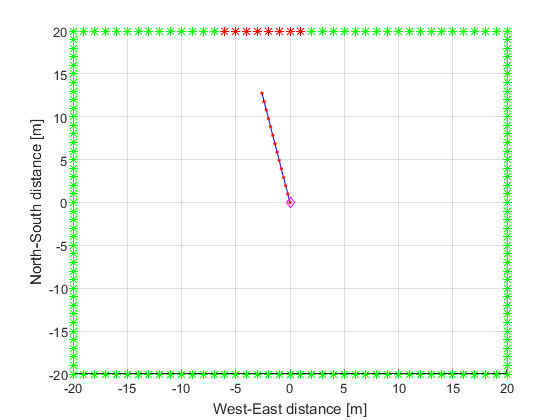
\includegraphics[width=0.9\linewidth]{\FIGDIR/21_Obstacle_detection.png} 
    \caption{Obstacle detection}
    \label{fig:21Obstacledetection}
    \end{subfigure}
    \begin{subfigure}{0.5\textwidth}
    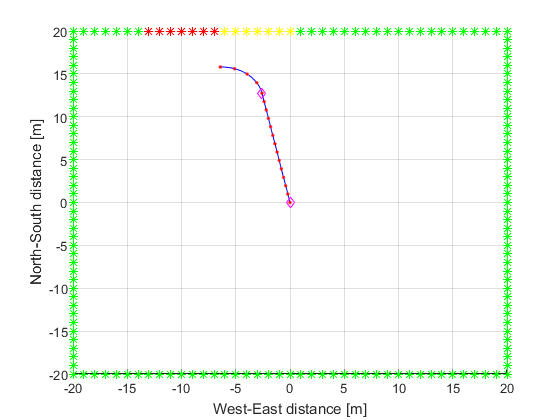
\includegraphics[width=0.9\linewidth]{\FIGDIR/22_Avoidance.png}
    \caption{Avoidance}
    \label{fig:22Avoidance}
    \end{subfigure}
    \\
    \begin{subfigure}{0.5\textwidth}
    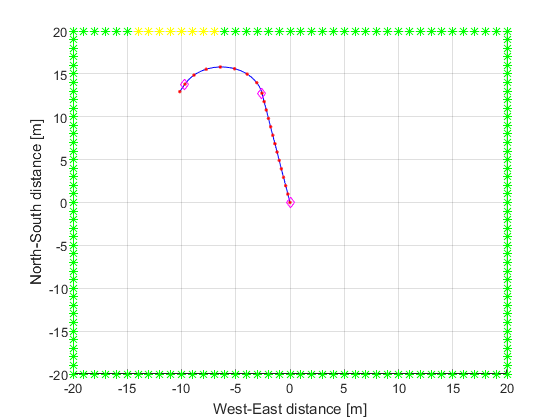
\includegraphics[width=0.9\linewidth]{\FIGDIR/23_End_of_avoidance.png} 
    \caption{End of avoidance}
    \label{fig:23Endofavoidance}
    \end{subfigure}
    \begin{subfigure}{0.5\textwidth}
    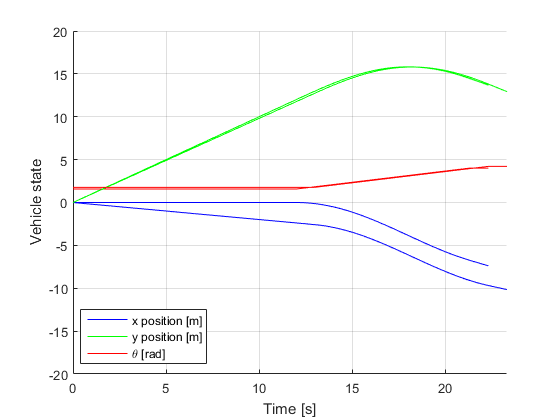
\includegraphics[width=0.9\linewidth]{\FIGDIR/24_Flight.png}
    \caption{Flight parameters}
    \label{fig:24Flightparameters}
    \end{subfigure}
\caption{Simulation results for left avoidance}
\label{fig:SimulationLeft}
\end{figure}

Starting parameters $x_v = 0$, $y_v = 0$, $\theta_v = \pi/2 + 0.2 $ in addition to initial parameters defined in table \ref{tab:simulationparameterss}. Vehicle is approaching wall from left side (\ref{fig:21Obstacledetection}). Multiple threats are detected, therefore control strategy $\Omega$ is restricted to turning left or right. Voting algorithm $\gamma$ counts more obstacles on right plane, therefore left avoidance maneuver is voted as most feasible. If avoidance maneuver will be selected as right turn, vehicle would crash into wall, because of greater turning radius and detection range $s_m$ is not sustainable to cover this gap. Design of crash distance function $d_c$ is strongly depending on robustness of voting algorithm $\gamma$. During avoidance maneuver (\ref{fig:22Avoidance}). obstacles are divined into obstacles in front of vehicle and obstacles behind vehicle. Multiple obstacles on the right side of vehicle are disallowing vehicle to turn right as can be seen in $\gamma$ table \ref{tab:avoidanceleft}. Avoidance maneuver ends when there is no threat $\mathscr{D} = \emptyset$ or there is no threat in vehicle heading $\forall o_i\in\mathscr{D},\delta_o=2$ as can be seen in figure \ref{fig:23Endofavoidance}. Evolution of state variables can be seen in figure \ref{fig:24Flightparameters}.

\begin{table}[H]
    \centering
    \begin{tabular}{|r||c|c|c|c|c|c|}
        \hline
        Right votes & 3 & 2 & 0  & 0  & 0  & 1\\ 
        \hline
        Left votes  & 5 & 9 & 13 & 13 & 13 & 12\\
        \hline
        \hline
        Decision    & L & L & L  & L  & L  & L\\
        \hline
    \end{tabular}
    \caption{Voting algorithm result for left avoidance}
    \label{tab:avoidanceleft}
\end{table}


\subsection{Right slide avoidance} 
\begin{figure}[H]
    \begin{subfigure}{0.5\textwidth}
    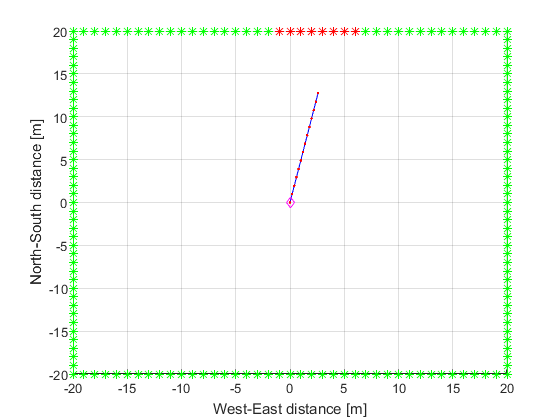
\includegraphics[width=0.9\linewidth]{\FIGDIR/25_Obstacle_detection.png} 
    \caption{Obstacle detection}
    \label{fig:25Obstacledetection}
    \end{subfigure}
    \begin{subfigure}{0.5\textwidth}
    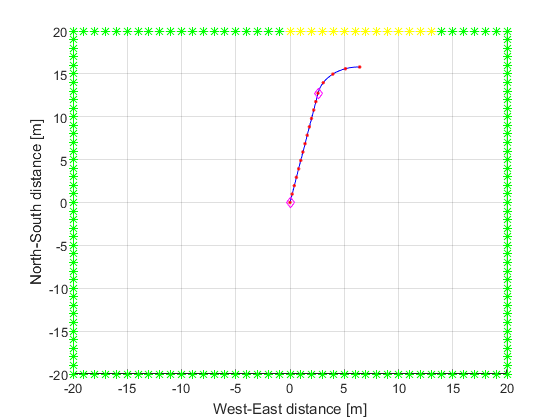
\includegraphics[width=0.9\linewidth]{\FIGDIR/26_Avoidance.png}
    \caption{Avoidance}
    \label{fig:26Avoidance}
    \end{subfigure}
    \\
    \begin{subfigure}{0.5\textwidth}
    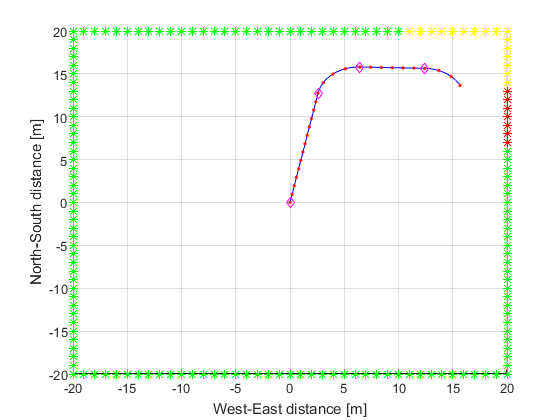
\includegraphics[width=0.9\linewidth]{\FIGDIR/27_End_of_avoidance.png} 
    \caption{End of avoidance}
    \label{fig:27Endofavoidance}
    \end{subfigure}
    \begin{subfigure}{0.5\textwidth}
    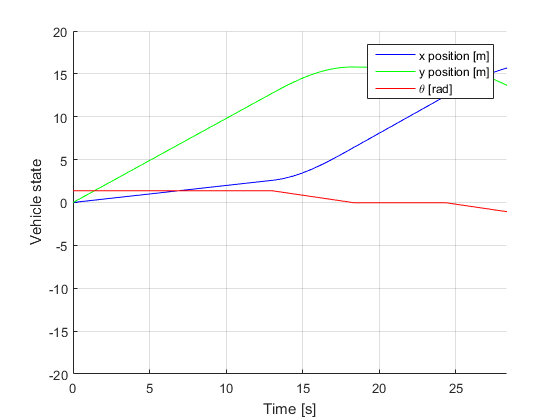
\includegraphics[width=0.9\linewidth]{\FIGDIR/28_Flight.png}
    \caption{Flight parameters}
    \label{fig:28Flightparameters}
    \end{subfigure}
\caption{Simulation results for right avoidance}
\label{fig:SimulationRight}
\end{figure}

Starting parameters $x_v = 0$, $y_v = 0$, $\theta_v = \pi/2 - 0.2 $ in addition to initial parameters defined in table \ref{tab:simulationparameterss}. Obstacle detection (\ref{fig:25Obstacledetection}) starts avoidance maneuver and restricst control strategy $\Omega$ to turn left or right. Because more threats $o_i\in\mathscr{D}$ are on left plane, voting algorithm $\gamma$ chooses to turn right. Voting algorithm decisions are summarized in table \ref{tab:avoidanceright}. Avoidance maneuver ends after quater-turn to right (\ref{fig:26Avoidance}). Vehicle moves along within wall until it detects threating obstacle in front $\delta_i=1$ and starts to turning right again (\ref{fig:27Endofavoidance}). Control strategy $\Omega$, voting algorithm $\gamma$ and crash distance function is deterministic. Decision time $t_{step}$ is fixed. The reason why vehicle behaves differently is numerical stability of $\cos,\sin,\arctan$ functions used in algorithm and unequal division of voting rule in $\gamma$ which favors left side. State vector evolution during maneuver is portrayed in figure \ref{fig:28Flightparameters}.

\begin{table}[H]
    \centering
    \begin{tabular}{|r||c|c|c|c|}
        \hline
        Right votes & 5 & 9 & 13 & 13\\
        \hline
        Left votes  & 5 & 2 & 0  & 0\\
        \hline\hline
        Decision    & R & R & R  & R\\
        \hline
    \end{tabular}
    \caption{Voting algorithm result for right avoidance}
    \label{tab:avoidanceright}
\end{table}

\subsection{Corner avoidance} 
\begin{figure}[H]
    \begin{subfigure}{0.5\textwidth}
    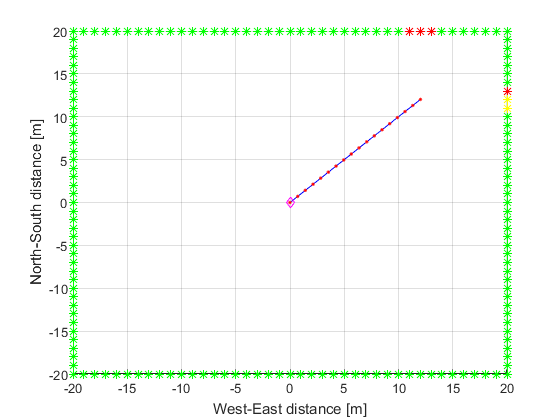
\includegraphics[width=0.9\linewidth]{\FIGDIR/29_Obstacle_detection.png} 
    \caption{Obstacle detection}
    \label{fig:29Obstacledetection}
    \end{subfigure}
    \begin{subfigure}{0.5\textwidth}
    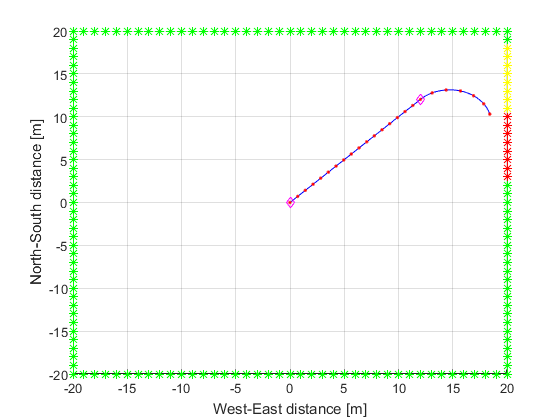
\includegraphics[width=0.9\linewidth]{\FIGDIR/30_Avoidance.png}
    \caption{Avoidance}
    \label{fig:30Avoidance}
    \end{subfigure}
    \\
    \begin{subfigure}{0.5\textwidth}
    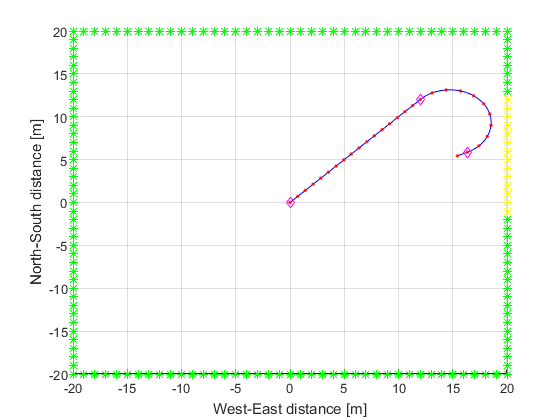
\includegraphics[width=0.9\linewidth]{\FIGDIR/31_End_of_avoidance.png} 
    \caption{End of avoidance}
    \label{fig:31Endofavoidance}
    \end{subfigure}
    \begin{subfigure}{0.5\textwidth}
    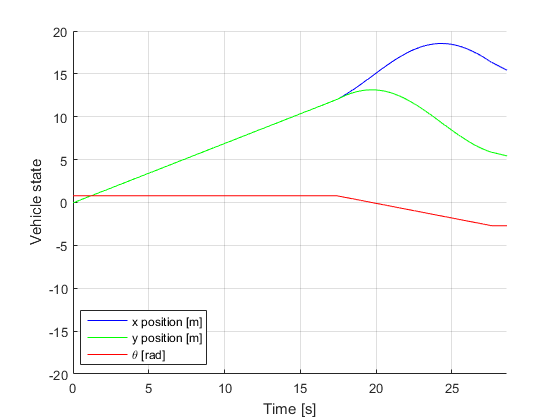
\includegraphics[width=0.9\linewidth]{\FIGDIR/32_Flight.png}
    \caption{Flight parameters}
    \label{fig:32Flightparameters}
    \end{subfigure}
\caption{Simulation results for corner avoidance}
\label{fig:SimulationCorner}
\end{figure}

Starting parameters $x_v = 0$, $y_v = 0$, $\theta_v = \pi/4$ in addition to initial parameters defined in table \ref{tab:simulationparameterss}. Obstacle detection in corner avoidance (\ref{fig:29Obstacledetection}), should detect same amount of problematic obstacles on the left and on the right side at first approach, but outcome is different, there are three $\delta_o=1$ threats on left and one $\delta_o=1$ threat plus one $\delta_o=2$ threat on the right. This disproportion is caused by $\arctan$ numerical instability. Voting algorithm $\gamma$ therefore chooses to turn right, because there is lesser amount of obstacles. During corner avoidance (\ref{fig:30Avoidance}) vehicle almost touches wall, enough place is provided by decision constant $s_m$ in crash distance function calculation (\ref{eq:smartdistancefunction}). End of avoidance (\ref{fig:31Endofavoidance}) is invoked when all threats $o_i\in\mathscr{D}$, have threat type assesed as $\delta_o=2$. Voting algorithm $\gamma$ decisions are summarized in table \ref{tab:avoidancecorner}. Evolution of vehicle states in time is portrayed in figure \ref{fig:32Flightparameters}.

\begin{table}[H]
    \centering
    \begin{tabular}{|r||c|c|c|c|c|c|c|c|c|c|}
        \hline
        Right votes & 6 & 15 & 15 & 13 & 11 & 11 & 14 & 16 & 12 & 10\\
        \hline
        Left votes  & 0 &  1 &  5 &  8 & 10 &  5 &  2 &  0 &  4 &  6\\
        \hline\hline
        Decision    & R & R  &  R &  R &  R &  R &  R &  R &  R &  R\\
        \hline
    \end{tabular}
    \caption{Voting algorithm result for corner avoidance}
    \label{tab:avoidancecorner}
\end{table}


\subsection{Long term avoidance} 
\begin{figure}[H]
    \begin{subfigure}{0.5\textwidth}
    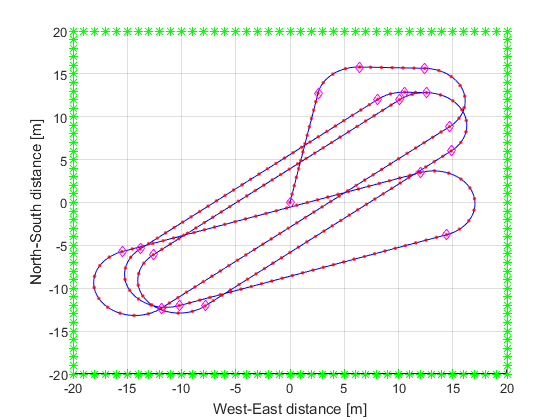
\includegraphics[width=0.9\linewidth]{\FIGDIR/33_Flight_trajectory.png} 
    \caption{Flight trajectory}
    \label{fig:33Flighttrajectory}
    \end{subfigure}
    \begin{subfigure}{0.5\textwidth}
    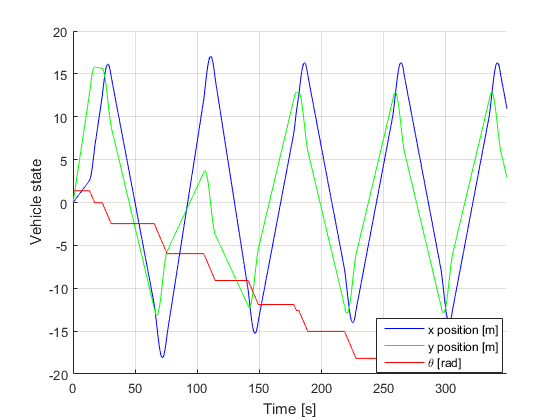
\includegraphics[width=0.9\linewidth]{\FIGDIR/34_Flight_parameters.png}
    \caption{Flight parameters}
    \label{fig:34Flightparameters}
    \end{subfigure}
\caption{Simulation results for long term avoidance}
\label{fig:Simulationlongterm}
\end{figure}

Starting parameters $x_v = 0$, $y_v = 0$, $\theta_v = \pi/2 - 0.2 $, given simulation time $t_sim =  400 s$, in addition to initial parameters defined in table \ref{tab:simulationparameterss}. All other partial maneuvers were successful. Because of multiple avoidance maneuvers, voting algorithm $\gamma$ is not shown in results, other decisions are not shown in results. Flight trajectory is displayed in figure \ref{fig:33Flighttrajectory}. Vehicle does not leave playground which is successful and it was moving in almost all areas of playground except north-west corner. Vehicle states evolution is portrayed in figure \ref{fig:34Flightparameters}. 